\documentclass[12pt,a4paper]{article}

\usepackage[serbian]{babel}

\usepackage{graphicx}
\usepackage{float}

\usepackage{listings}
\usepackage{xcolor} % for setting colors

% text width and height
\textwidth 16cm
\textheight 23cm

% distance from the top
\voffset -1.5cm

% distance from the left
\hoffset 0cm
\oddsidemargin 0mm

% distance from the bottom
\footskip 1.5cm

\linespread{1}

% set the default code style
\lstset{language=python,
     xleftmargin=20pt,
      basicstyle=\ttfamily,
      morekeywords={to, downto, then},
      keywordstyle=\color{blue}\ttfamily,
      stringstyle=\color{red}\ttfamily,
      commentstyle=\color{green}\ttfamily,
      morecomment=[l][\color{magenta}]{\#},
      numbers=left,
      basicstyle=\small
}

\title{Analiza skupa podataka Food choices}
\author{Tijana Jevti\' c \\ Jelena Mrdak}

\setlength\parindent{0pt}

\begin{document}
\maketitle
\begin{abstract}
Skup podataka Food choices predstavlja skup odgovora studenata sa koledza na odredjena pitanja vezana za njihove navike u ishrani. Dakle, podaci su dobijeni anketiranjem 126 studenata na 60 pitanja razlicitog tipa. Neka pitanja se konkretno ticu njihovih preferenca vezanih za hranu, njihovih navika, dok se kroz ostala dobija vise informacija o njihovom socio-ekonomskom statusu. Sve to zajedno cini bogat skup podataka iz kog se moze zakljuciti dosta zanimljivih pravilnosti.

Koliko se dana\v snji studenti brinu o ishrani i koliko znaju o hrani? Da li njihove navike ste\v cene jo\v s u detinjstvu uti\v cu na to kako se danas hrane? Koliko njihove kulinarske ve\v stine uti\v cu na na\v cin na koji se hrane? Zasto jedu i da li je jedini odgovor zbog gladi? Da li odgovor na prethodno pitanje zavisi od pola?

Na ova i jo\v s mnogobrojna pitanja, poku\v sa\' cemo da odgovorimo u ovom radu.
\end{abstract}

\tableofcontents

\section{Opis skupa podataka}
Skup podataka - datoteka food\_coded.csv sadrzi sadrzi 60 razlicitih atributa. Podaci su, za sada, neocisceni. U nastavku cemo pomenuti svaki od atributa kako bi se citalac upoznao sa skupom podataka, a posebnu paznju cemo posvetiti onima koje koristimo u istrazivanju.

\begin{itemize}
  \item GPA - numeri\v cki, prosek na fakultetu\\
  \item Pol - kategori\v cki\\
    \textbf{1} - \v zensko\\
    \textbf{2} - mu\v sko
  \item Doru\v cak - koja od 2 ponudjene slike ispitanike vise asocira na dorucak\\
    Ispitanicima je ponu\dj ena slika pahuljica i krofne i treba da ka\v zu \v sta ih asocira na doru\v cak\\
    \textbf{1} - pahuljice\\
    \textbf{2} - krofna 
  \item Procena kalorija u jednom par\v cetu piletine\\
    \textbf{1} - 265\\ 
    \textbf{2} - 430\\
    \textbf{3} - 610\\
    \textbf{4} - 720
  \item Da li je bitna koli\v cina kalorija koja se konzumira dnevno\\
    \textbf{1} - ne znam koliko kalorija treba konzumirati dnevno\\
    \textbf{2} - uop\v ste nije bitno\\
    \textbf{3} - umereno je bitno\\
    \textbf{4} - veoma je bitno
  \item Procena kalorija u kolacu iz Starbucks-a\\
    \textbf{1} - 107 cal\\ 
    \textbf{2} - 315 cal\\ 
    \textbf{3} - 420 cal\\ 
    \textbf{4} - 980 cal
  \item Kafa - koja od 2 ponudjene slike ispitanike vise asocira na kafu\\
  \item Hrana za utehu\\ - koja hrana asocira ispitanike na dom i lepe uspomene, cini ih srecnim
    Ispitanici treba da navedu izmedju 3 i 5 razlicitih jela.\\
  \item Zasto posezu za hranom za utehu \\
    Ispitanici treba da navedu do 3 razloga za\v sto jedu hranu za utehu? (npr. tuga, sre\' ca, bes)\\
  \item Hrana za utehu - kodirana\\
   \textbf{1} - stres\\
   \textbf{2} - dosada\\
   \textbf{3} - depresija\\
   \textbf{4} - glad\\
   \textbf{5} - lenjost\\
   \textbf{6} - hladno vreme \\
   \textbf{7} - sre\'  ca\\ 
   \textbf{8} - gledanje televizije\\
   \textbf{9} - ni\v sta od navedenog\\
   \item Kuvanje - koliko ispitanici cesto kuvaju\\
    \textbf{1} - svakog dana\\
    \textbf{2} - nekoliko dana nedeljno\\
    \textbf{3} - koliko cesto mogu, ali retko\\
    \textbf{4} - jedino za praznike\\
    \textbf{5} - nikada\\
  \item Koji tip kuhinje su jeli kad su bili mali\\
    \textbf{1} - americka\\
    \textbf{2} - meksicka/spanska\\
    \textbf{3} - korejska/azijska\\
    \textbf{4} - indijska\\
    \textbf{5} - americka sa internacionalnim jelima\\
    \textbf{6} - ostalo\\
  \item Trenutna dijeta\\
  \item Trenutna dijeta - kodirano od 1 do 4\\
  \item Koju sliku asociraju sa picem\\
  \item Kako se ishrana promenila od kada su na koledzu\\
  \item Kako se ishrana promenila\\
    \textbf{1} - na losija\\
    \textbf{2} - na bolje\\
    \textbf{3} - isto\\
    \textbf{4} - nije sigurno\\
  \item Kako se ishrana promenila u terminima toga sta jedu\\
  \item Prejedanje - koliko se ispitanici cesto prejedaju tokom nedelje\\
    \textbf{1} - nikad\\
    \textbf{2} - 1 do 2 puta\\
    \textbf{3} - 2 do 3 puta\\
    \textbf{4} - 3 do 5 puta\\
    \textbf{5} - svaki dan\\
  \item Zaposlenje - da li su zaposleni
    \textbf{1} - da, puno radno vreme\\
    \textbf{2} - da, poluradno vreme\\
    \textbf{3} - ne\\
    \textbf{4} - drugo\\
  \item 
  \item Vezbanje - koliko puta nedeljno vezbaju\\
    \textbf{1} - svakodnevno\\
    \textbf{2} - 2 do 3 puta\\
    \textbf{3} - jednom\\
    \textbf{4} - ponekad\\
    \textbf{5} - nikad\\
  \item Ocevo obrazovanje\\
  \item Oceva profesija\\
  \item Omiljena vrsta kuhinje\\
  \item Omiljena vrsta kuhinje - kodirano\\
  \item Omiljena hrana - kuvana ili kupljena\\
    \textbf{1} - kuvana kod kuce\\
    \textbf{2} - kupljena u prodavnici\\
    \textbf{3} - oba\\
  \item Omiljena hrana iz detinjstva\\
  \item Koja od 2 slike ih vise asocira sa krompiricima\\
  \item Voce - koliko je verovatno da ce pojesti voce tokom dana\\
    \textbf{1} - vrlo verovatno\\
    \textbf{2} - ne toliko verovatno\\
    \textbf{3} - onako\\
    \textbf{4} - verovatno\\
    \textbf{5} - vrlo verovatno\\
  \item Godina na koledzu\\
  \item Grcka hrana - koliko je verovatno da bi je jeli\\
  \item Koliko se zdravo osecaju od 1 do 10\\
  \item Sta je, po njihovim recima, zdrav obrok\\
  \item Sta je, po njihovim recima, idealna ishrana\\
  \item Idealna ishrana - kodirano\\
  \item Zarada - koliko zaradjuju godisnje\\
    \textbf{1} - manje od 15 000 dolara\\
    \textbf{2} - 15 001 - 30 000 dolara\\
    \textbf{3} - 30 001 - 50 000 dolara\\
    \textbf{4} - 50 001 - 70 000 dolara\\
    \textbf{5} - 70 001 - 100 000 dolara\\
    \textbf{6} - vise od 100 000 dolara\\
  \item Indijska hrana - koliko je verovatno da bi je jeli\\
  \item Italijanska hrana - koliko je verovatno da bi je jeli\\
  \item Koliko je zivot lep od 1 do 10\\
  \item Bracni zivot\\
    \textbf{1} - slobodan/slobodna\\
    \textbf{2} - u vezi\\
    \textbf{3} - zivi sa partnerom\\
    \textbf{4} - udat/ozenjen\\
    \textbf{5} - razveden/a\\
    \textbf{6} - udovica\\
  \item Sta bi posluzili kao veceru prijatelju\\
  \item Majcino obrazovanje\\
  \item Majcina profesija\\
  \item Koliko cesto proveravaju kolicinu kalorija hrane koje konzumiraju\\
  \item Da li zive ili ne na kampusu\\
  \item Koliko puta nedeljno roditelji kuvaju\\
    \textbf{1} - skoro svaki dan\\
    \textbf{2} - 2 do 3 puta\\
    \textbf{3} - 1 do 2 puta\\
    \textbf{4} - za vreme odmora\\
    \textbf{5} - nikad\\
  \item Placanje obroka - koliko bi novca potrosili na obrok\\
  \item Persijska hrana - koliko je verovatno da bi je jeli\\
  \item Procena sopstvene tezine\\
    \textbf{1} - vitak/vitka\\
    \textbf{2} - vrlo utreniran/utrenirana\\
    \textbf{3} - tacno kako treba\\
    \textbf{4} - pomalo debeo/debela\\
    \textbf{5} - debeo/debela\\
    \textbf{6} - ne razmisljam o tome kada mislim o sebi\\
  \item Koja od 2 slike ih vise asocira sa supom\\
  \item Sport - da li se bave sportom\\
    \textbf{1} - da\\
    \textbf{2} - ne\\
    \textbf{99} - bez odgovora\\
  \item Tajlandska hrana - koliko je verovatno da bi je jeli\\
  \item Koliko tortilja ima kalorija\\
  \item Koliko guska ima kalorija\\
  \item Sport - kojim sportom se bave\\
  \item Povrce - koliko je verovatno da jedu povrce na dnevnoj bazi\\
  \item Vitamini - da li uzimaju dodatne vitamine\\
  \item Koliko vafl ima kalorija\\
  \item Tezina (u funtama: 1kg = 2.20462 funti)\\
\end{itemize}

\section{Primer klasifikacije}

Odredi\' cemo klasifikaciju na osnovu atributa comfort\_food\_reasons\_coded, cook i eating\_out, dok \' ce nam ciljni atribut biti weight.\\

Najpre \' cemo u\v citati podatke i prikazati prvih pet redova.\\

\begin{lstlisting}[mathescape=true]
df = pd.read_csv('./food-choices/food_coded.csv')
print('\n{}'.format(df.head()))
\end{lstlisting}

\begin{verbatim}
  GPA  Gender  breakfast ... waffle_calories                    weight
0   2.4       2          1 ...            1315                       187
1 3.654       1          1 ...             900                       155
2   3.3       1          1 ...             900  I'm not answering this.
3   3.2       1          1 ...            1315             Not sure, 240
4   3.5       1          1 ...             760                       190
\end{verbatim}

Mo\v zemo uraditi osnovnu statistiku za svaku kolonu.

\begin{lstlisting}[mathescape=true]
print("\nStatistike skupa:\n{}".format(df.describe()))
\end{lstlisting}

\begin{verbatim}
Statistike skupa:
           Gender   breakfast  calories_chicken ... veggies_day    vitamins
count  125.000000  125.000000        125.000000 ...  125.000000  125.000000
mean     1.392000    1.112000        577.320000 ...    4.008000    1.512000
std      0.490161    0.316636        131.214156 ...    1.081337    0.501867
min      1.000000    1.000000        265.000000 ...    1.000000    1.000000
25%      1.000000    1.000000        430.000000 ...    3.000000    1.000000
50%      1.000000    1.000000        610.000000 ...    4.000000    2.000000
75%      2.000000    1.000000        720.000000 ...    5.000000    2.000000
max      2.000000    2.000000        720.000000 ...    5.000000    2.000000
\end{verbatim}

Za algoritam koji \v zelimo da primenimo, izdvoji\' cemo slede\' ce atribute: comfort\_food\_reasons\_coded, cook, eating\_out i weight.

\begin{lstlisting}[mathescape=true]
target_attribute = 'weight'
attribute_1 = 'comfort_food_reasons_coded'
attribute_2 = 'cook'
attribute_3 = 'eating_out'

df = df[[attribute_1, attribute_2, attribute_3, target_attribute]]
\end{lstlisting}

\begin{verbatim}
   comfort_food_reasons_coded  cook  eating_out                    weight
0                         9.0   2.0           3                       187
1                         1.0   3.0           2                       155
2                         1.0   1.0           2  I'm not answering this.
3                         2.0   2.0           2             Not sure, 240
4                         1.0   1.0           2                       190
\end{verbatim}

Kao \v sto mo\v zemo primetiti, nisu sve vrednosti celobrojne. Zato \' cemo obrisati sve redove koji sadr\v ze NaN-ove ili stringove u nekoj od ove \v cetiri kolone. Tako\dj e, vrednosti u koloni weight \' cemo transformisati. Preslika\' cemo ih u skup $\{0, 1, 2\}$.


\begin{lstlisting}[mathescape=true]
df = df.replace('nan', np.nan)
df = df.dropna()


df = df[df[target_attribute].apply(lambda x: str(x).isdigit())]

df.reset_index(drop=True, inplace=True)

df[attribute_1] = df.comfort_food_reasons_coded.astype(int)
df[attribute_2] = df.cook.astype(int)
df[attribute_3] = df.eating_out.astype(int)
df[target_attribute] = df.weight.astype(int)

changes = {}
weight = df[target_attribute].unique()
for w in weight:
    if int(w) <150:
        changes[w] = 0
    elif int(w) < 190:
        changes[w] = 1
    else:
        changes[w] = 2

df[target_attribute] = df[target_attribute].replace(changes)
\end{lstlisting}

\begin{verbatim}
   comfort_food_reasons_coded  cook  eating_out  weight
0                           9     2           3       1
1                           1     3           2       1
2                           1     1           2       2
3                           4     3           1       2
4                           1     2           2       1
\end{verbatim}

Sada \' cemo izvr\v siti podelu skupa na test i trening skup.

\begin{lstlisting}
X = df[[attribute_1, attribute_2, attribute_3]]
y = df[[target_attribute]]

X_train, X_test, y_train, y_test = train_test_split(X, y, test_size=0.3)
print("\nVelicina skupa za obucavanje: {}".format(X_train.size))
print("Velicina skupa za testiranje: {}".format(X_test.size))
\end{lstlisting}

\begin{verbatim}
Velicina skupa za obucavanje: 207
Velicina skupa za testiranje: 90
\end{verbatim}

Po\v sto smo izvr\v sili podelu skupa, primeni\' cemo algoritam za klasifikaciju - $k$ najbli\v zih suseda.

\begin{lstlisting}
clf = KNeighborsClassifier(5, 'distance')

# Treniramo model
clf.fit(X_train, y_train.values.ravel())

# Vrsimo predikciju
y_test_predicted = clf.predict(X_test)
y_train_predicted = clf.predict(X_train)

# Izracunavamo preciznost
train_acc = clf.score(X_train, y_train)
test_acc = clf.score(X_test, y_test)
print('train preciznost: {}'.format(train_acc))
print('test preciznost: {}'.format(test_acc))
\end{lstlisting}

\begin{verbatim}
train preciznost: 0.7536231884057971
test preciznost: 0.7
\end{verbatim}

Izve\v staj i matricu konfuzije mo\v zemo dobiti na slede\' ci na\v cin:

\begin{lstlisting}
test_rep = sklearn.metrics.classification_report(y_test, y_test_predicted)
train_rep = sklearn.metrics.classification_report(y_train, y_train_predicted)
print("\nTest izvestaj:\n{}".format(test_rep))
print("Trening izvestaj:\n{}".format(train_rep))

train_conf = sklearn.metrics.confusion_matrix(y_train, y_train_predicted)
test_conf = sklearn.metrics.confusion_matrix(y_test, y_test_predicted)
print("Matrica konfuzije za skup za obucavanje:\n{}".format(train_conf))
print("\nMatrica konfuzije za skup za testiranje:\n{}".format(test_conf))
\end{lstlisting}

\begin{verbatim}
Test izvestaj:
             precision    recall  f1-score   support

          0       0.67      0.91      0.77        11
          1       0.77      0.67      0.71        15
          2       0.50      0.25      0.33         4

avg / total       0.70      0.70      0.68        30

Trening izvestaj:
             precision    recall  f1-score   support

          0       0.74      0.86      0.79        29
          1       0.73      0.81      0.77        27
          2       1.00      0.38      0.56        13

avg / total       0.78      0.75      0.74        69

Matrica konfuzije za skup za obucavanje:
[[25  4  0]
 [ 5 22  0]
 [ 4  4  5]]

Matrica konfuzije za skup za testiranje:
[[10  1  0]
 [ 4 10  1]
 [ 1  2  1]]
\end{verbatim}

\section{Vizuelizacija podataka}


\begin{lstlisting}
fig = plt.figure()
ax = fig.add_subplot(111, projection='3d')


colors = ['green', 'blue','red']
for (v, color) in zip(weight, colors):
    subsamples = df.loc[df[target_attribute] == v]
    ax.scatter(subsamples[attribute_1], 
               subsamples[attribute_2], 
               subsamples[attribute_3],
               color=color, s=70, alpha=0.3)

ax.set_xlabel('comfort_food_reasons_coded')
ax.set_ylabel('cook')
ax.set_zlabel('eating_out')
plt.show()
\end{lstlisting}

\begin{figure}[H]
  \centering
  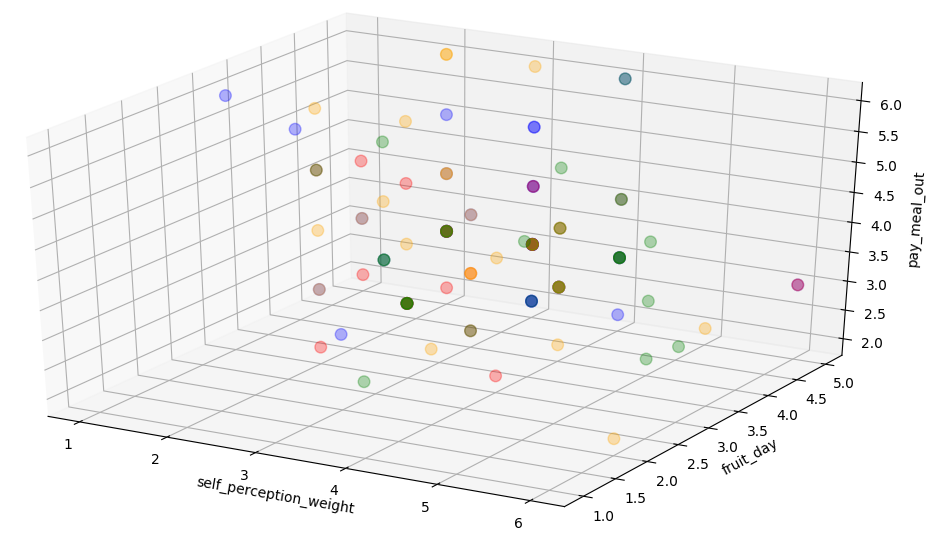
\includegraphics[width=15cm]{3dgrafik.png}
\end{figure}


\begin{thebibliography}{9}
  \bibitem{knjiga1}Knjiga1
  \bibitem{knjiga2}Knjiga2
\end{thebibliography}

\end{document}
